%Created with command:
%"/home/josh/Teaching/trunk/Utilities/makeexam" "Quiz 3" "Please show all work.  You may not use a calculator." "../LatchesAndFlipFlops/Assessments/latch_flip-flop.tex" "../LatchesAndFlipFlops/Assessments/d_flip-flop_clock.tex" "../StateMachines/Assessments/state_machine_partition.tex" "../StateMachines/Assessments/number_of_flipflops.tex"
\documentclass{article}
\usepackage[T1]{fontenc}
\usepackage{arev}
\usepackage{longtable}
\usepackage[hmargin=2cm,vmargin=2cm]{geometry}
\usepackage{graphicx}
\usepackage{listings}
\setlength{\parindent}{0pt}
\title{Quiz 3}
\date{}
\begin{document}
\maketitle
Please show all work.  You may not use a calculator. (14 points total)
\begin{longtable}[l]{rp{17cm}}
%file: ../LatchesAndFlipFlops/Assessments/latch_flip-flop.tex
1.&\begin{minipage}[t]{\linewidth}(2 pt) Briefly explain the key difference between a latch and a flip-flop. \\

Solution: \\ \\
A flip-flop operates using a clock signal, a latch does not. \\
\end{minipage}\\
\medskip
%file: ../LatchesAndFlipFlops/Assessments/d_flip-flop_clock.tex
2.&\begin{minipage}[t]{\linewidth}(4 pt) The following figure is a partial implementation of a D flip-flop using two D latches.  Correctly connect the clock input (CLK) within the circuit.  Note that you may need to use one or more logic gates to complete this problem. \\ \\
\begin{center}
  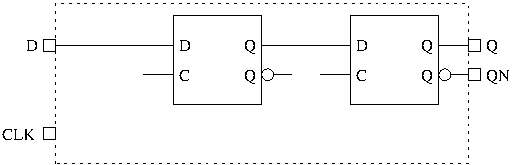
\includegraphics{../LatchesAndFlipFlops/Assessments/DFlipFlopLogicNoClock}
\end{center}

Solution: \\ \\
\begin{center}
  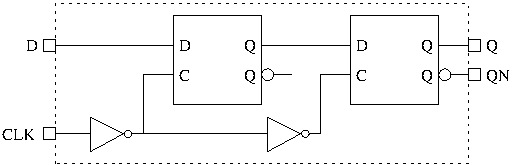
\includegraphics{../LatchesAndFlipFlops/Assessments/DFlipFlopLogic}
\end{center}
\end{minipage}\\
\medskip
%file: ../StateMachines/Assessments/state_machine_partition.tex
3.&\begin{minipage}[t]{\linewidth}(4 pt) Graphically divide the following state machine circuit diagram into the three basic parts of a state machine: the next-state logic, the state memory, and the output logic.  Which named signals in the diagram are the excitation signals?
\begin{center}
  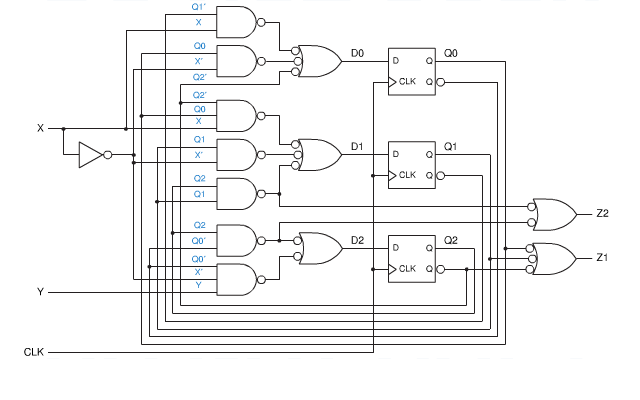
\includegraphics[scale=0.7]{../StateMachines/Assessments/Wakerly_7_43}
\end{center}

Solution: \\ \\
D0, D1, and D2 are the excitation signals.\\ \\
\begin{center}
  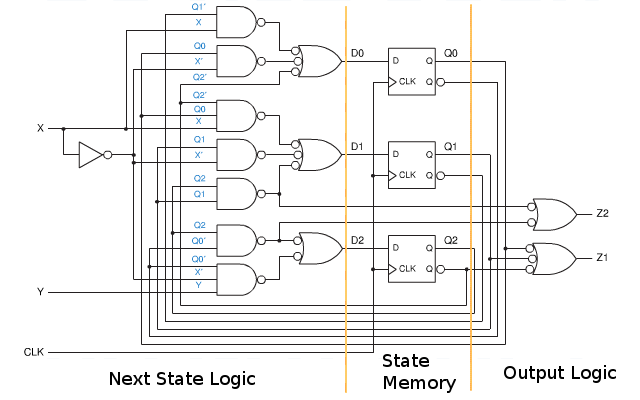
\includegraphics[scale=0.7]{../StateMachines/Assessments/Wakerly_7_43_annotated}
\end{center}
\end{minipage}\\
\medskip
%file: ../StateMachines/Assessments/number_of_flipflops.tex
4.&\begin{minipage}[t]{\linewidth}(4 pt) Given a state machine with 10 states:\\
(a) What is the minimum number of flip-flops required to fully implement the state memory for this state machine?\\
(b) Without knowing anything else about the state machine, how many flip-flops are required to allow the simplest excitation equations to be written?\\ \\

Solution: \\ \\
(a) At least 4 flip-flops are required, since they will provide $2^1=16$ states, where 3 flip-flops will provide on $2^3=8$ states.\\
(b) If we use one flip-flop to represent each state (10 flip-flops total), then the excitation equations will be very simple.\\
\end{minipage}\\
\medskip
\end{longtable}
\end{document}